\Csection{Постановка задачи}

Требуется реализовать некоторую виртуальную модель какой-либо геометрической фигуры. Виртуальная модель должна описывать фигуру в трёхмерном пространстве, дополнительно на саму модель налагается задача преобразования координат в зависимости от углов поворота. Описание фигуры выполнено в виде двух массивов $K$ и $L$. Массив $K$ --- двумерный массив размерности $n \times 3$, где $n$ --- количество точек, описывающие фигуру, а 3 --- координаты $X$, $Y$ и $Z$ в декартовой системе координат. Массив $L$ --- плоский одномерный массив размерности $1 \times 2k$, где $k$ --- количество связей между какими-либо точками фигуры. 

В качестве примера возьмём куб с вершинами $A$, $B$, $C$, $D$, $E$, $F$, $G$ и $H$.

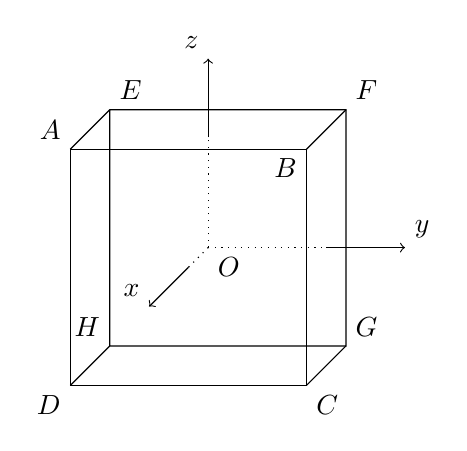
\begin{tikzpicture}
\draw (0, 0) node [above left] {$A$} -- (3, 0) node [below left] {$B$} -- (3, -3) node [below right] {$C$} -- (0, -3) node [below left] {$D$} -- (0, 0);
\draw (0, 0) -- (0.5, 0.5) node [above right] {$E$} -- (3.5, 0.5) node [above right] {$F$} -- (3.5, -2.5) node [above right] {$G$} -- (0.5, -2.5) node [above left] {$H$} -- (0.5, 0.5);
\draw (3, 0) -- (3.5, 0.5);
\draw (3, -3) -- (3.5, -2.5);
\draw (0, -3) -- (0.5, -2.5);
\draw [dotted] (1.75, -1.25) node [below right] {$O$} -- (1.75, 0.15);
\draw [->] (1.75, 0.15) -- (1.75, 1.15) node [above left] {$z$};
\draw [dotted] (1.75, -1.25) -- (1.5, -1.5);
\draw [->] (1.5, -1.5) -- (1.0, -2) node [above left] {$x$};
\draw [dotted] (1.75, -1.25) -- (3.25, -1.25);
\draw [->] (3.25, -1.25) -- (4.25, -1.25) node [above right] {$y$};
\end{tikzpicture}

Тогда, если допустить что начало декартовой системы координат находится в центре масс куба, то координаты куба можно задать следующим образом: $A(t, -t, t)$, $B(t, t, t)$, $C(t, t, -t)$, $D(t, -t, -t)$, $E(-t, -t, t)$, $F(-t, t, t)$, $G(-t, t, -t)$ и $H(-t, -t, -t)$. В виде массива данные координаты можно записать так:

$K =
\begin{pmatrix}
t & -t & t \\
t & t & t \\
t & t & -t \\
t & -t & -t \\
-t & -t & t \\
-t & t & t \\
-t & t & -t \\
-t & -t & -t
\end{pmatrix}$

В этой матрице строка 0 --- это точка $A$, 1 --- точка $B$, ..., 7 --- точка $H$ (отсчёт идёт с нуля).

Связи между точками образуются следующими парами: $(A, B)$, $(A, E)$, $(A, D)$, $(B, F)$, $(B, C)$, $(C, G)$, $(C, D)$, $(D, H)$, $(E, F)$, $(E, H)$, $(F, G)$ и $(G, H)$. Причём пары $(A, B)$ и $(B, A)$ --- это одна и та же пара. В виде матрицы-строки связи можно записать так:

$L =
\begin{pmatrix}
0, 1, 0, 4, 0, 3, 1, 5, 1, 2, 2, 6, 2, 3, 3, 7, 4, 5, 4, 7, 5, 6, 6, 7
\end{pmatrix}$

Если отсчитывать элементы индексов с нуля то образуются связи $(L(0), L(1)) = (A, B)$, $(L(2), L(3)) = (A, E)$, ..., $(L(6), L(7)) = (G, H)$. Поскольку в массиве $L$ перечислены пары, то количество элементов в $L$ может быть только чётным.

Помимо этого объект трёхмерной модели должен содержать сведения об углах поворота исходной системы координат. В данном случае этих углов три штуки: угол поворота $\alpha$ вокруг оси $OX$, угол поворота $\beta$ вокруг оси $OY$ и угол поворота $\gamma$ вокруг оси $OZ$. Положительным направлением поворота считается: для угла $\alpha$ --- поворот оси $OY$ к оси $OZ$, для угла $\beta$ --- поворот оси $OZ$ к $OX$ и для угла $\gamma$ --- поворот оси $OX$ к оси $OY$.

Новая система координат (полученная после поворота старой системы координат) в старой системе координат будет выражаться так:

$$x' = (x \cos{\gamma} - y \sin{\gamma}) \cos{\beta} + z \sin{\beta}$$

$$y' = (y \cos{\gamma} + x \sin{\gamma}) \cos{\alpha} - z \sin{\alpha}$$

$$z' = (z \cos{\alpha} + y \sin{\alpha}) \cos{\beta} - x \sin{\beta}$$

где $x'$, $y'$ и $z'$ --- это новые координаты точки в старой системе координат полученные после поворота, $x$, $y$ и $z$ --- это начальные координаты точки в старой системе координат.
